%!TEX root = ../main.tex 

\section{Pourquoi une impédance?}

\subsection{Power Factor}
\begin{frame}{Différence de phase entre réactances}
    \begin{figure}
        \centering
        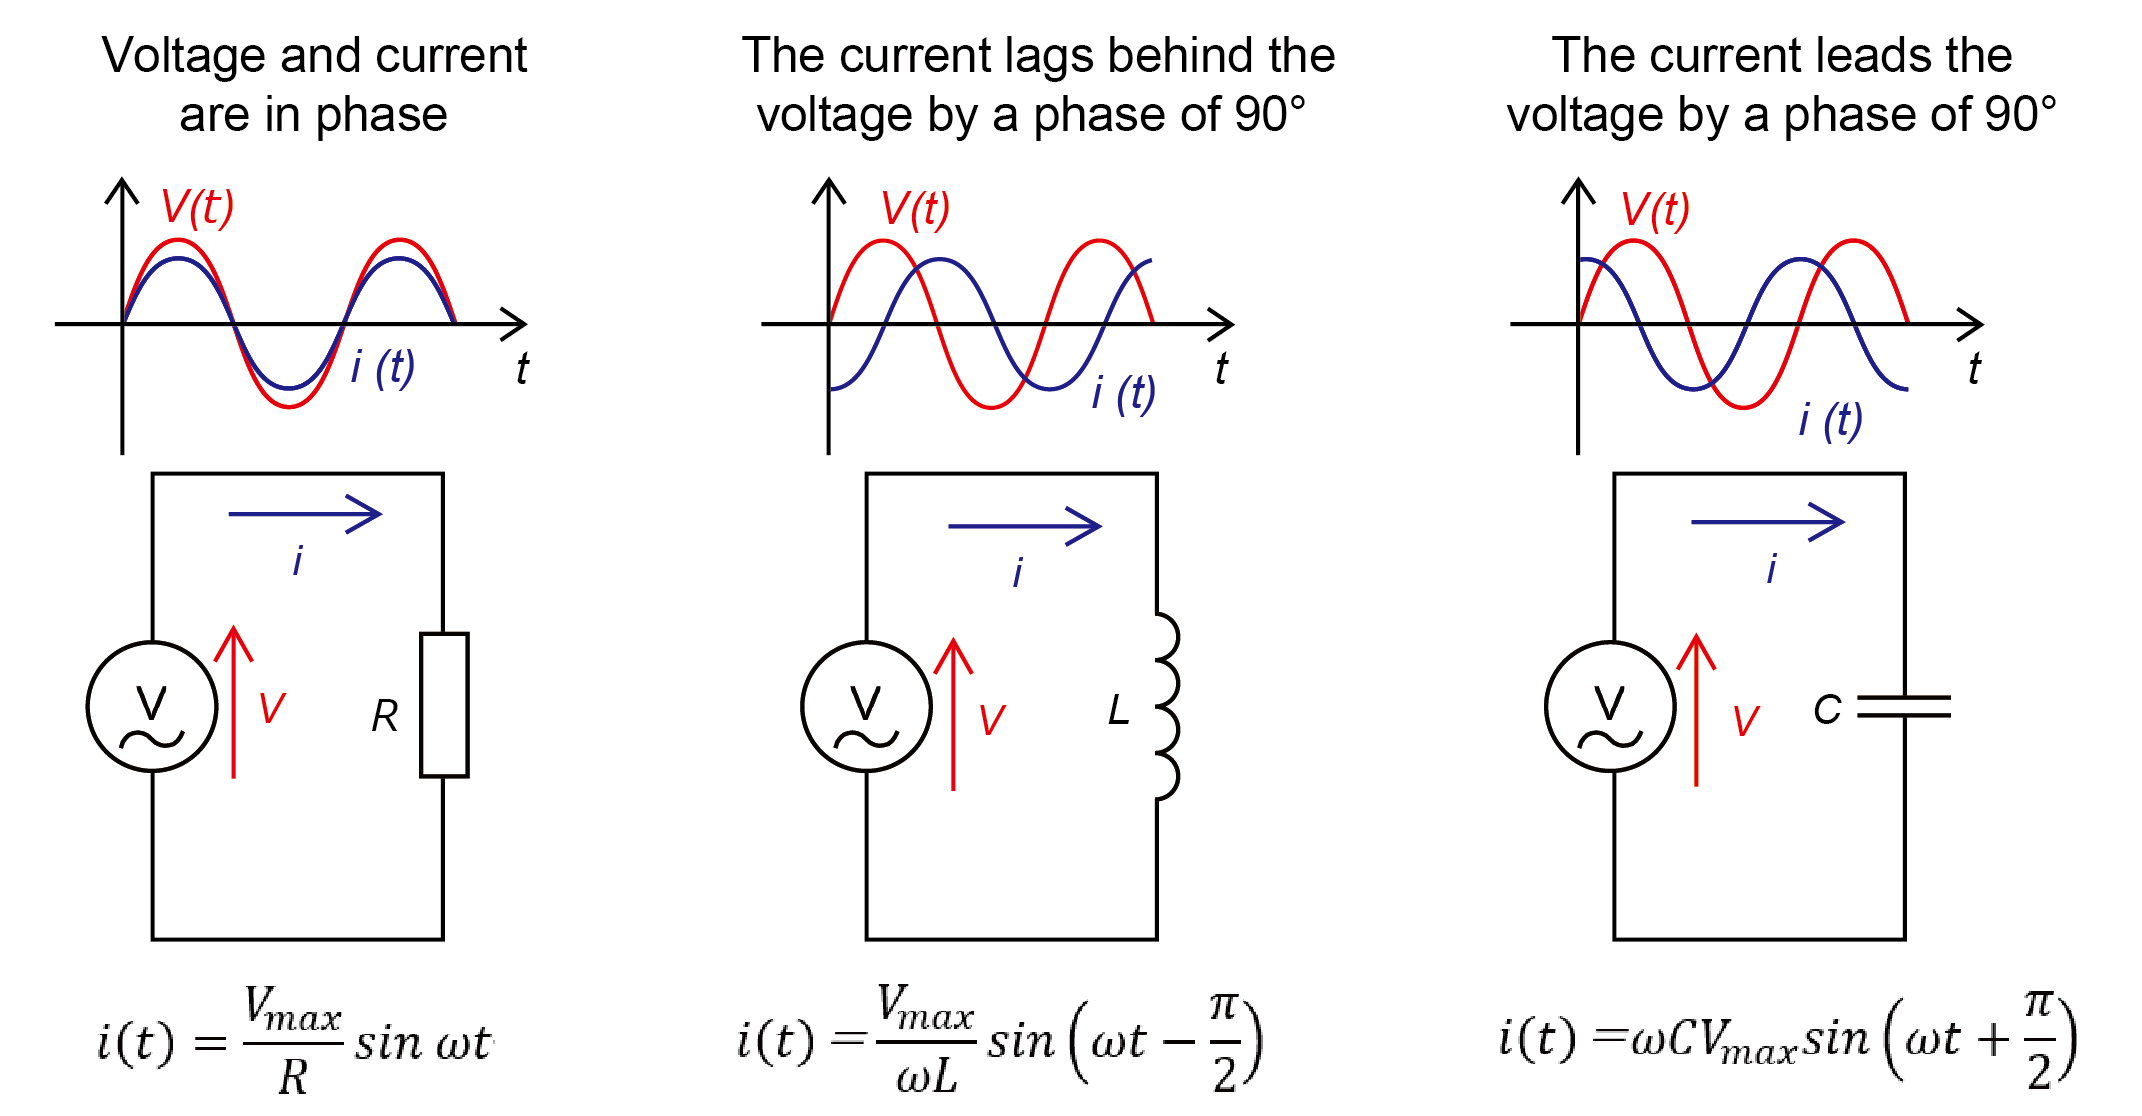
\includegraphics[width=\textwidth]{pictures/Phase_Difference_Between_Impedance_and_Current.png}
    \end{figure}
\end{frame}

\begin{frame}{Power Factor}
    \begin{columns}
        \begin{column}{0.5\textwidth}
            \begin{itemize}
                \item Ratio du \textit{vrai} power ($kW$) au power \textit{apparent} ($kVA$).
                \item Avec impédance imaginaire vient puissance imaginaire
                \item Seule la puissance réelle est utile
            \end{itemize}
            \begin{figure}
                \centering
                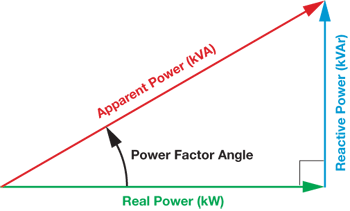
\includegraphics[width=\textwidth]{pictures/power-factor.png}
            \end{figure}
        \end{column}
        \begin{column}{0.5\textwidth}
            \begin{figure}
                \centering
                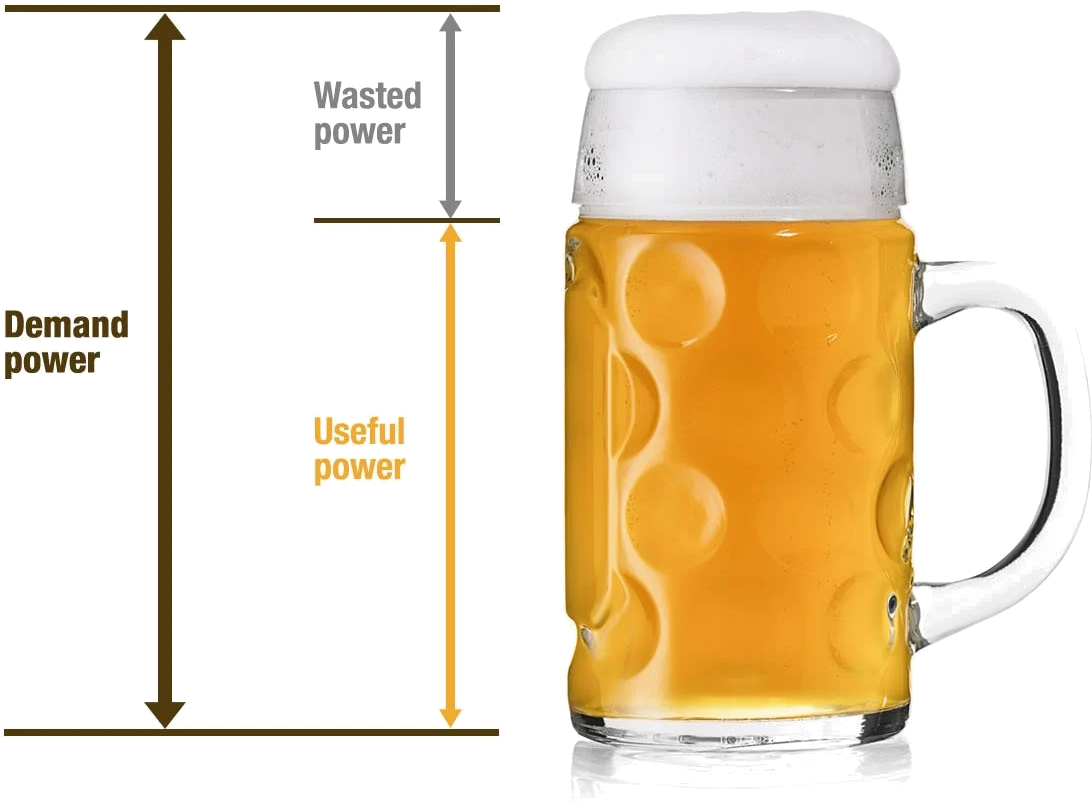
\includegraphics[width=\textwidth]{pictures/power-factor-beer.png}
            \end{figure}
        \end{column}
    \end{columns}
\end{frame}


\subsection{Réflexions sur un circuit ouvert}

\begin{frame}{Ligne de transmission - Circuit Ouvert}
    \begin{center}

    \Large{$i = \frac{V}{Z_0}$}
    
    \resizebox{0.9\textwidth}{!}{
    \begin{circuitikz}[american voltages]
        \draw [thick]
        (0,0) to [short, *-*] (8,0)
        to [open, -*] (8,4)
        (0,0) to [open, v<=$5V$] (0,4)
        to [short, *- ,i=$i$, a=$100mA$] (4,4)
        to [european resistor, l=$Z_0$, a=$50\Omega$] (6, 4)
        to [short, -*] (8,4)
        ;
        \draw[thick, dashed]
        (8, 4) to [short] (8, 3)
        to [short, a=\mbox{$i_L=0A$}] (8, 2)
        to [short, a=\mbox{$Z_L = \infty$}] (8, 1)
        to [short] (8, 0);
    \end{circuitikz}
    }
    \end{center}
\end{frame}

\begin{frame}{Circuit Ouvert - Onde à envoyer}
    \begin{center}
        \begin{tikzpicture}
            \begin{axis}[
                axis lines = left,
                xlabel = \(t\),
                ylabel = \(V\),
                ymax = 3.3,
                xmax = 10,
            ]
            \addplot [
                domain=0:10,
                thick,
                color=red,
            ]
            coordinates
            {(0, 0) (1, 0) (1.5, 1) (6, 1) (6.5, 0) (10, 0)};
            \addlegendentry{\(Input\ Voltage\)}
            \end{axis}
        \end{tikzpicture}
    \end{center}
\end{frame}

\begin{frame}
    \begin{columns}
        \begin{column}{0.5\textwidth}
            \begin{itemize}
                \item Impulsion très courte
                \item (Impulsion fini avant réflexion)
                \bigskip
                \item Circuit ouvert au bout
                \item Signal réfléchit avec 2x amplitude
            \end{itemize}
        \end{column}
        \begin{column}{0.5\textwidth}
            \begin{center}
            \resizebox{\textwidth}{!}{%
                \begin{tikzpicture}
                    \begin{axis}[
                        axis lines = left,
                        xlabel = \(t\),
                        ylabel = \(V\),
                        ymax = 3.3,
                        xmax = 10,
                    ]
                    \addplot [
                        domain=0:10,
                        very thick,,
                        color=red,
                    ]
                    coordinates
                    {(0, 0) (1, 0) (1.5, 1) (6, 1) (6.5, 0) (10, 0)};
                    \addlegendentry{\(Input\ Voltage\)}
                    \end{axis}
                \end{tikzpicture}
            }
            \resizebox{0.9\textwidth}{!}{
                \begin{circuitikz}[american voltages]
                    \draw [thick]
                    (0,0) to [short, *-*] (8,0)
                    to [open, -*] (8,4)
                    (0,0) to [open, v<=$V$] (0,4)
                    to [short, *- ,i_=$i$] (4,4)
                    to [european resistor, l_=$Z_0$] (6, 4)
                    to [short, -*] (8,4);
                \end{circuitikz}
            }
            \end{center}
        \end{column}
    \end{columns}
\end{frame}

\begin{frame}{Circuit Ouvert}
    \begin{center}
        \begin{tikzpicture}
            \begin{axis}[
                axis lines = left,
                xlabel = \(p\),
                ylabel = \(V\),
                ymax = 3.3,
                xmax = 10,
                title={t = 2},
            ]
            \addplot [
                domain=0:10,
                very thick,,
                color=red,
            ]
            coordinates
            {(0, 1) (1, 1) (1.25, 0) (10, 0)};
            \end{axis}
        \end{tikzpicture}
    \end{center}
\end{frame}

\begin{frame}{Circuit Ouvert}
    \begin{center}
        \begin{tikzpicture}
            \begin{axis}[
                axis lines = left,
                xlabel = \(p\),
                ylabel = \(V\),
                ymax = 3.3,
                xmax = 10,
                title={t = 3},
            ]
            \addplot [
                domain=0:10,
                very thick,,
                color=red,
            ]
            coordinates
            {(0, 1) (7, 1) (7.25, 0) (10, 0)};
            \end{axis}
        \end{tikzpicture}
    \end{center}
\end{frame}

\begin{frame}{Circuit Ouvert}
    \begin{center}
        \begin{tikzpicture}
            \begin{axis}[
                axis lines = left,
                xlabel = \(p\),
                ylabel = \(V\),
                ymin = 0,
                ymax = 3.3,
                xmax = 10,
                title={t = 4},
            ]
            \addplot [
                domain=0:10,
                very thick,,
                color=red,
            ]
            coordinates
            {(0, 1) (8, 1) (8.25, 2) (10, 2)};
            \end{axis}
        \end{tikzpicture}
    \end{center}
\end{frame}

\begin{frame}{Circuit Ouvert}
    \begin{center}
        \begin{tikzpicture}
            \begin{axis}[
                axis lines = left,
                xlabel = \(p\),
                ylabel = \(V\),
                ymin = 0,
                ymax = 3.3,
                xmax = 10,
                title={t = 7},
            ]
            \addplot [
                domain=0:10,
                very thick,,
                color=red,
            ]
            coordinates
            {(0, 0) (1, 0) (1.25, 1) (3, 1) (3.25, 2) (10, 2)};
            \end{axis}
        \end{tikzpicture}
    \end{center}
\end{frame}

\begin{frame}{Circuit Ouvert}
    \begin{center}
        \begin{tikzpicture}
            \begin{axis}[
                axis lines = left,
                xlabel = \(p\),
                ylabel = \(V\),
                ymin = 0,
                ymax = 3.3,
                xmax = 10,
                title={t = 8},
            ]
            \addplot [
                domain=0:10,
                very thick,,
                color=red,
            ]
            coordinates
            {(0, 1) (2, 1) (2.25, 2) (10, 2)};
            \end{axis}
        \end{tikzpicture}
    \end{center}
\end{frame}

\begin{frame}{Circuit Ouvert}
    \begin{center}
        \begin{tikzpicture}
            \begin{axis}[
                axis lines = left,
                xlabel = \(p\),
                ylabel = \(V\),
                ymin = 0,
                ymax = 3.3,
                xmax = 9,
                title={t = 10},
            ]
            \addplot [
                domain=0:10,
                very thick,,
                color=red,
            ]
            coordinates
            {(0, 1) (8, 1) (8.25, 2) (10, 2)};
            \end{axis}
        \end{tikzpicture}
    \end{center}
\end{frame}

\begin{frame}{Circuit Ouvert}
    \begin{center}
        \begin{tikzpicture}
            \begin{axis}[
                axis lines = left,
                xlabel = \(p\),
                ylabel = \(V\),
                ymin = 0,
                ymax = 3.3,
                xmax = 10,
                title={t = 10},
            ]
            \addplot [
                domain=0:10,
                very thick,,
                color=red,
            ]
            coordinates
            {(0, 1) (6, 1) (6.25, 0) (10, 0)};
            \end{axis}
        \end{tikzpicture}
    \end{center}
\end{frame}

\begin{frame}{Circuit Ouvert}
    \begin{center}
        \begin{tikzpicture}
            \begin{axis}[
                axis lines = left,
                xlabel = \(p\),
                ylabel = \(V\),
                ymin = 0,
                ymax = 3.3,
                xmax = 10,
                title={t = 11},
            ]
            \addplot [
                domain=0:10,
                very thick,,
                color=red,
            ]
            coordinates
            {(0, 1) (1, 1) (1.25, 0) (10, 0)};
            \end{axis}
        \end{tikzpicture}
    \end{center}
\end{frame}

\begin{frame}{Circuit Ouvert - Vraie forme d'onde}
    \begin{columns}
        \begin{column}{0.5\textwidth}
            \begin{center}
            \resizebox{\textwidth}{!}{%
                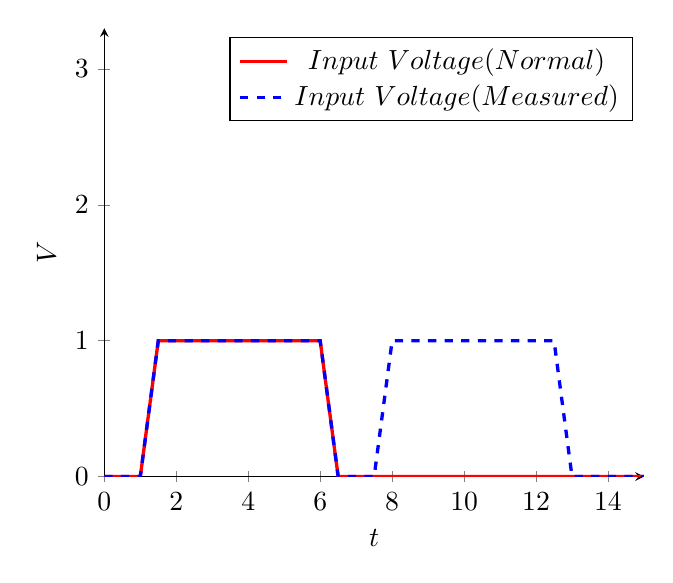
\begin{tikzpicture}
                    \begin{axis}[
                        axis lines = left,
                        xlabel = \(t\),
                        ylabel = \(V\),
                        ymax = 3.3,
                        xmax = 15,
                    ]
                    \addplot [
                        domain=0:15,
                        very thick,
                        color=red,
                    ]
                    coordinates
                    {(0, 0) (1, 0) (1.5, 1) (6, 1) (6.5, 0) (15, 0)};
                    \addlegendentry{\(Input\ Voltage (Normal)\)}

                    \addplot [
                        domain=0:15,
                        very thick,
                        color=blue,
                        style=dashed,
                    ]
                    coordinates
                    {(0, 0) (1, 0) (1.5, 1) (6, 1) (6.5, 0) (7.5, 0) (8, 1) (12.5, 1) (13, 0) (15, 0)};
                    \addlegendentry{\(Input\ Voltage (Measured)\)}
                    \end{axis}
                \end{tikzpicture}
            }
            \end{center}
        \end{column}

        \begin{column}{0.5\textwidth}
            \begin{center}
            \resizebox{\textwidth}{!}{%
                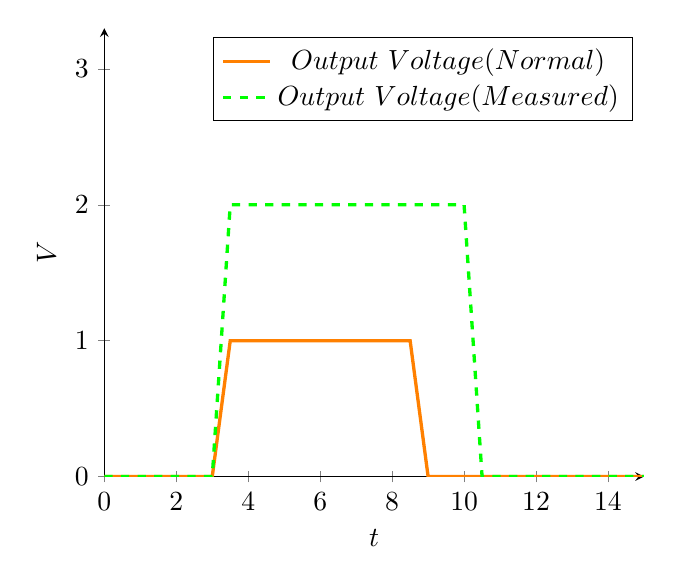
\begin{tikzpicture}
                    \begin{axis}[
                        axis lines = left,
                        xlabel = \(t\),
                        ylabel = \(V\),
                        ymax = 3.3,
                        xmax = 15,
                    ]
                    \addplot [
                        domain=0:15,
                        very thick,,
                        color=orange,
                    ]
                    coordinates
                    {(0, 0) (3, 0) (3.5, 1) (8.5, 1) (9, 0) (15, 0)};
                    \addlegendentry{\(Output\ Voltage (Normal)\)}

                    \addplot [
                        domain=0:15,
                        very thick,,
                        color=green,
                        style=dashed
                    ]
                    coordinates
                    {(0, 0) (3, 0) (3.5, 2) (10, 2) (10.5, 0) (15, 0)};
                    \addlegendentry{\(Output\ Voltage (Measured)\)}
                    \end{axis}
                \end{tikzpicture}
            }
            \end{center}
        \end{column}
    \end{columns}
\end{frame}

\begin{frame}{Circuit Ouvert - Oscilloscope}
    \begin{columns}
        \begin{column}{0.6\textwidth}
            \begin{itemize}
                \item Oscilloscope à l'entrée
                \bigskip
                \item Réflexion en phase avec signal
                \item Pulse suivi d'un autre
                \item Délai = temps aller-retour du signal
                \bigskip
                \item Peut endommager la load
            \end{itemize}
        \end{column}
        
        \begin{column}{0.4\textwidth}
            \begin{figure}
                \centering
                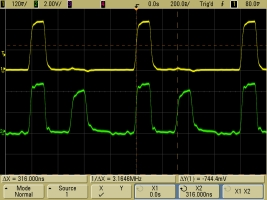
\includegraphics[width=\textwidth]{pictures/open-circuit-pulse-reflection.png}
            \end{figure}
        \end{column}
    \end{columns}
\end{frame}



\subsection{Réflexions sur un circuit ouvert 2}


\begin{frame}{Circuit Ouvert 2 - Onde à envoyer}
    \begin{columns}
        \begin{column}{0.5\textwidth}
            \begin{center}
            \resizebox{\textwidth}{!}{
                \begin{tikzpicture}
                    \begin{axis}[
                        axis lines = left,
                        xlabel = \(t\),
                        ylabel = \(V\),
                        ymax = 3.3,
                        xmax = 15,
                    ]
                    \addplot [
                        domain=0:15,
                        thick,
                        color=red,
                    ]
                    coordinates
                    {(0, 0) (1, 0) (1.5, 1) (12, 1) (12.5, 0) (15, 0)};
                    \addlegendentry{\(Input\ Voltage\)}
                    \end{axis}
                \end{tikzpicture}
            }
            \end{center}
        \end{column}
        \begin{column}{0.5\textwidth}
            \resizebox{\textwidth}{!}{
                \begin{circuitikz}[american voltages]
                    \draw [thick]
                    (0,0) to [short, *-*] (8,0)
                    to [open, -*] (8,4)
                    (0,0) to [open, v<=$V$] (0,4)
                    to [short, *- ,i_=$i$] (4,4)
                    to [european resistor, l_=$Z_0$] (6, 4)
                    to [short, -*] (8,4);
                \end{circuitikz}
            }
        \end{column}
    \end{columns}
\end{frame}

\begin{frame}{Circuit Ouvert 2 - Vraie forme d'onde}
    \begin{center}
        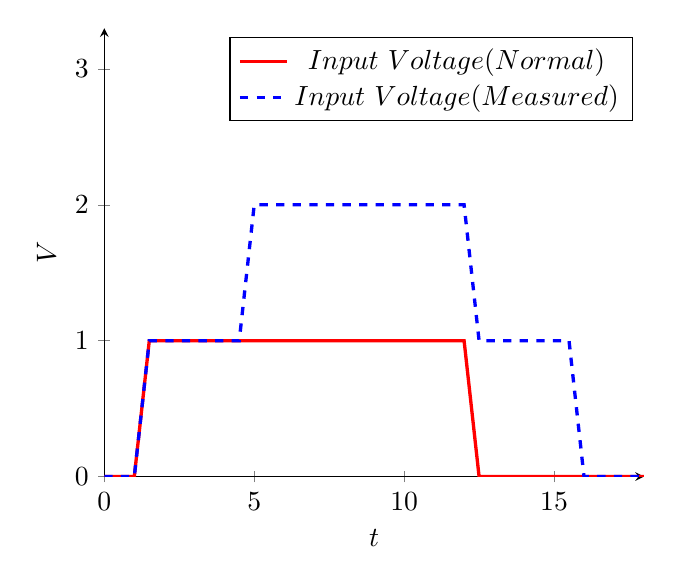
\begin{tikzpicture}
            \begin{axis}[
                axis lines = left,
                xlabel = \(t\),
                ylabel = \(V\),
                ymax = 3.3,
                xmax = 18,
            ]
            \addplot [
                domain=0:18,
                very thick,
                color=red,
            ]
            coordinates
            {(0, 0) (1, 0) (1.5, 1) (12, 1) (12.5, 0) (18, 0)};
            \addlegendentry{\(Input\ Voltage (Normal)\)}

            \addplot [
                domain=0:18,
                very thick,
                color=blue,
                style=dashed,
            ]
            coordinates
            {(0, 0) (1, 0) (1.5, 1) (4.5, 1) (5, 2) (12, 2) (12.5, 1) (15.5, 1) (16, 0) (18, 0)};
            \addlegendentry{\(Input\ Voltage (Measured)\)}
            \end{axis}
        \end{tikzpicture}
    \end{center}
\end{frame}

\begin{frame}{Circuit Ouvert 2 - Oscilloscope}
    \begin{columns}
        \begin{column}{0.6\textwidth}
            \begin{itemize}
                \item Oscilloscope à l'entrée
                \bigskip
                \item Pulse plus long
                \item Délai de propagation $ps$ \textless pulse
                \bigskip
                \item Peut endommager la load
                \item Peut endommager la source
            \end{itemize}
        \end{column}
        
        \begin{column}{0.4\textwidth}
            \begin{figure}
                \centering
                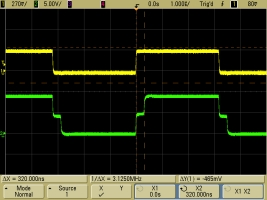
\includegraphics[width=\textwidth]{pictures/open-circuit-pulse-reflection-2.png}
            \end{figure}
        \end{column}
    \end{columns}
\end{frame}

\subsection{Que se passe-t'il?}
\begin{frame}{Coefficient Gamma - Diapo de maths surprise!}
    \begin{center}
        $\Gamma = \dfrac{V_r}{V_i} = -\dfrac{I_r}{I_i}$\\
        \vspace{10pt}
        $\Gamma = \dfrac{Z_L - Z_0}{Z_L + Z_0}$\\
    \end{center}
    \vspace{3.33mm}
    \begin{columns}
        \begin{column}{0.33\textwidth}<2->
            \begin{center}
                $Z_L = Z_0$\\
                \vspace{10pt}
                $\Gamma = \dfrac{0}{Z_L + Z_0}$\\
                \vspace{10pt}
                $\Gamma = 0$\\
                \vspace{5pt}
                $V_r = 0$\\
                \vspace{5pt}
                Pas de réflexion!
            \end{center}
        \end{column}
        \begin{column}{0.33\textwidth}<3->
            \begin{center}
                $Z_L = \infty$\\
                \vspace{10pt}
                $\Gamma = \dfrac{\infty}{\infty}$\\
                \vspace{10pt}
                $\Gamma = 1$\\
                \vspace{5pt}
                $V_r = V_i$\\
                \vspace{5pt}
                Même tension réfléchie que rentrante
            \end{center}
        \end{column}
        \begin{column}{0.33\textwidth}<4->
            \begin{center}
                $Z_L = 0$\\
                \vspace{10pt}
                $\Gamma = -\dfrac{Z_0}{Z_0}$\\
                \vspace{10pt}
                $\Gamma = -1$\\
                \vspace{5pt}
                $V_r = -V_i$\\
                \vspace{5pt}
                Tension réfléchie négative?
            \end{center}
        \end{column}
    \end{columns}
\end{frame}


\begin{frame}{Circuit Fermé - Analogie}
    \begin{figure}
        \centering
        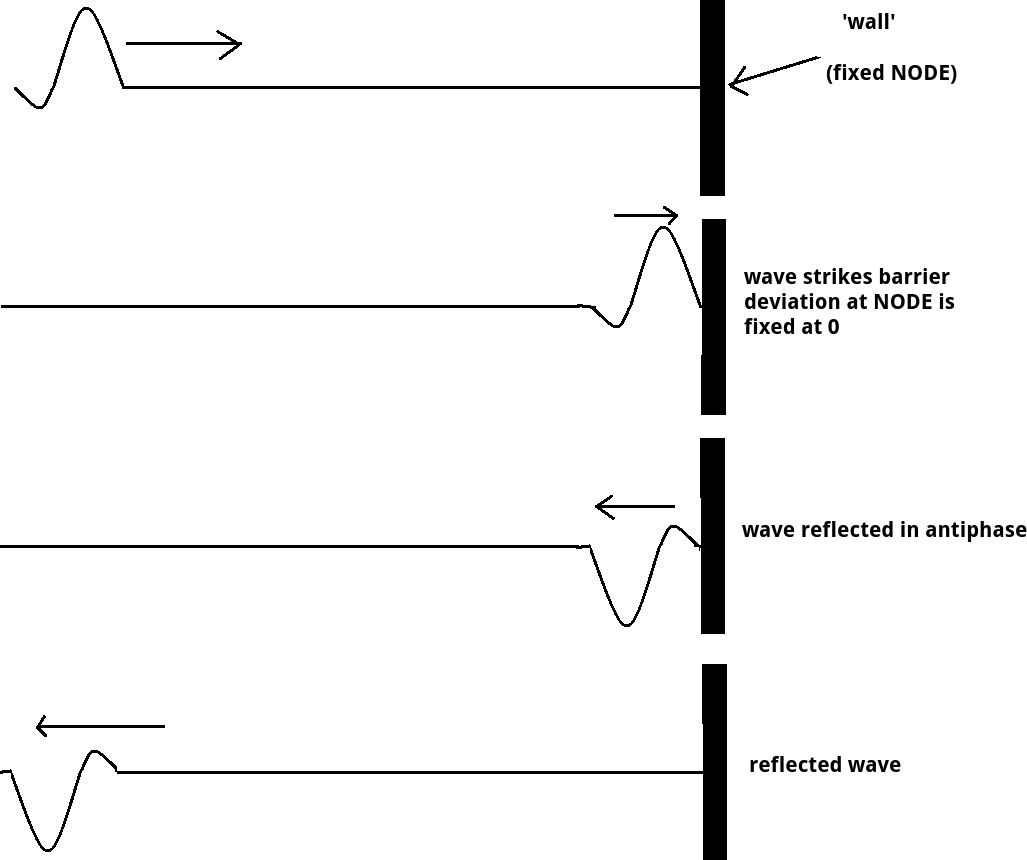
\includegraphics[width=0.8\textwidth, height=0.75\textheight, keepaspectratio]{pictures/closed-circuit-pulse-reflection-analogy.png}
    \end{figure}
\end{frame}

\begin{frame}{Mismatch d'impédance}
    \animategraphics[autoplay, controls, loop, width=\linewidth]{12}{pictures/partial-reflection/partial-reflection-}{0}{51}
\end{frame}


\subsection{Réflexions sur un circuit fermé}

\begin{frame}{Réflexions sur un circuit fermé}
    \begin{columns}
        \begin{column}{0.5\textwidth}
            \begin{itemize}
                \item Impulsion courte
                \bigskip
                \item Circuit fermé au bout
                \item Signal négatif réfléchit
            \end{itemize}
        \end{column}
        \begin{column}{0.5\textwidth}
            \begin{center}
            \resizebox{!}{0.45\textheight}{%
                \begin{tikzpicture}
                    \begin{axis}[
                        axis lines = left,
                        xlabel = \(t\),
                        ylabel = \(V\),
                        ymin = -2,
                        ymax = 2,
                        xmax = 10,
                    ]
                    \addplot [
                        domain=0:10,
                        very thick,,
                        color=red,
                    ]
                    coordinates
                    {(0, 0) (1, 0) (1.5, 1) (3, 1) (3.5, 0) (10, 0)};
                    \addlegendentry{\(Input\ Voltage\)}
                    \end{axis}
                \end{tikzpicture}
            }
            \resizebox{0.9\textwidth}{!}{
                \begin{circuitikz}[american voltages]
                \draw [thick]
                (0,0) to [short, *-] (8,0)
                to [resistor, l=$Z_L$, a=$0\Omega$] (8, 4)
                (0,0) to [open, v<=$5V$] (0,4)
                to [short, *- ,i=$i$, a=$100mA$] (4,4)
                to [european resistor, l=$Z_0$, a=$50\Omega$] (6, 4)
                to [short, -] (8,4)
                ;
                \end{circuitikz}
            }
            \end{center}
        \end{column}
    \end{columns}
\end{frame}

\begin{frame}{Circuit Fermé}
    \begin{center}
        \begin{tikzpicture}
            \begin{axis}[
                axis lines = left,
                xlabel = \(p\),
                ylabel = \(V\),
                ymin = -2,
                ymax = 2,
                xmax = 10,
                title={t = 2},
            ]
            \addplot [
                domain=0:10,
                very thick,
                color=red,
            ]
            coordinates
            {(0, 1) (1, 1) (1.25, 0) (10, 0)};
            \end{axis}
        \end{tikzpicture}
    \end{center}
\end{frame}


\begin{frame}{Circuit Fermé}
    \begin{center}
        \begin{tikzpicture}
            \begin{axis}[
                axis lines = left,
                xlabel = \(p\),
                ylabel = \(V\),
                ymin = -2,
                ymax = 2,
                xmax = 10,
                title={t = 4},
            ]
            \addplot [
                domain=0:10,
                very thick,
                color=red,
            ]
            coordinates
            {(0, 1) (8, 1) (8.25, -1) (10, -1)};
            \end{axis}
        \end{tikzpicture}
    \end{center}
\end{frame}

\begin{frame}{Circuit Fermé}
    \begin{center}
        \begin{tikzpicture}
            \begin{axis}[
                axis lines = left,
                xlabel = \(p\),
                ylabel = \(V\),
                ymin = -2,
                ymax = 2,
                xmax = 10,
                title={t = 5},
            ]
            \addplot [
                domain=0:10,
                very thick,
                color=red,
            ]
            coordinates
            {(0, 1) (1, 1) (1.25, -1) (10, -1)};
            \end{axis}
        \end{tikzpicture}
    \end{center}
\end{frame}

\begin{frame}{Circuit Fermé - Vraie forme d'onde}
    \begin{center}
        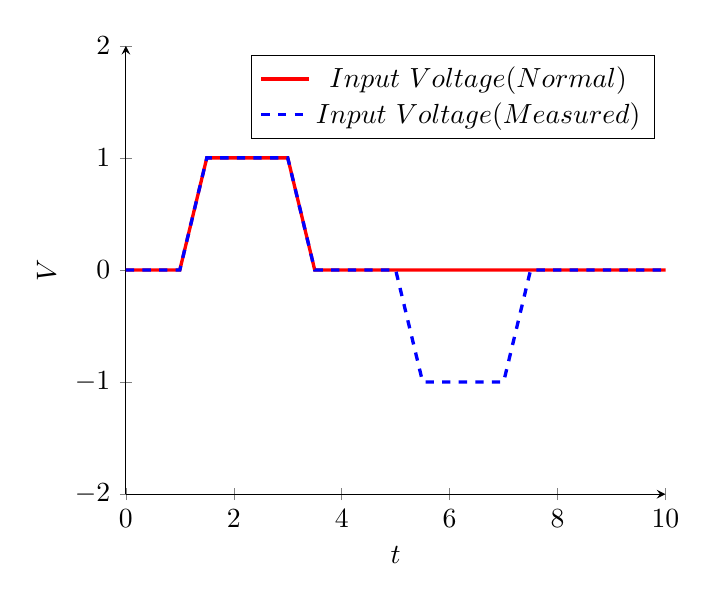
\begin{tikzpicture}
            \begin{axis}[
                axis lines = left,
                xlabel = \(t\),
                ylabel = \(V\),
                ymin = -2,
                ymax = 2,
                xmax = 10,
            ]
            \addplot [
                domain=0:10,
                very thick,
                color=red,
            ]
            coordinates
            {(0, 0) (1, 0) (1.5, 1) (3, 1) (3.5, 0) (10, 0)};
            \addlegendentry{\(Input\ Voltage (Normal)\)}

            \addplot [
                domain=0:18,
                very thick,
                color=blue,
                style=dashed,
            ]
            coordinates
            {(0, 0) (1, 0) (1.5, 1) (3, 1) (3.5, 0) (5, 0) (5.5, -1) (7, -1) (7.5, 0) (10, 0)};
            \addlegendentry{\(Input\ Voltage (Measured)\)}
            \end{axis}
        \end{tikzpicture}
    \end{center}
\end{frame}

\begin{frame}{Circuit Fermé - Oscilloscope}
    \begin{columns}
        \begin{column}{0.6\textwidth}
            \begin{itemize}
                \item Oscilloscope à l'entrée
                \bigskip
                \item Pulse court suivi d'un pulse négatif
                \item Même durée
                \item Délai de propagation $ps$ \textless pulse
                \bigskip
                \item Peut endommager la load
                \item Peut endommager la source
            \end{itemize}
        \end{column}
        
        \begin{column}{0.4\textwidth}
            \begin{figure}
                \centering
                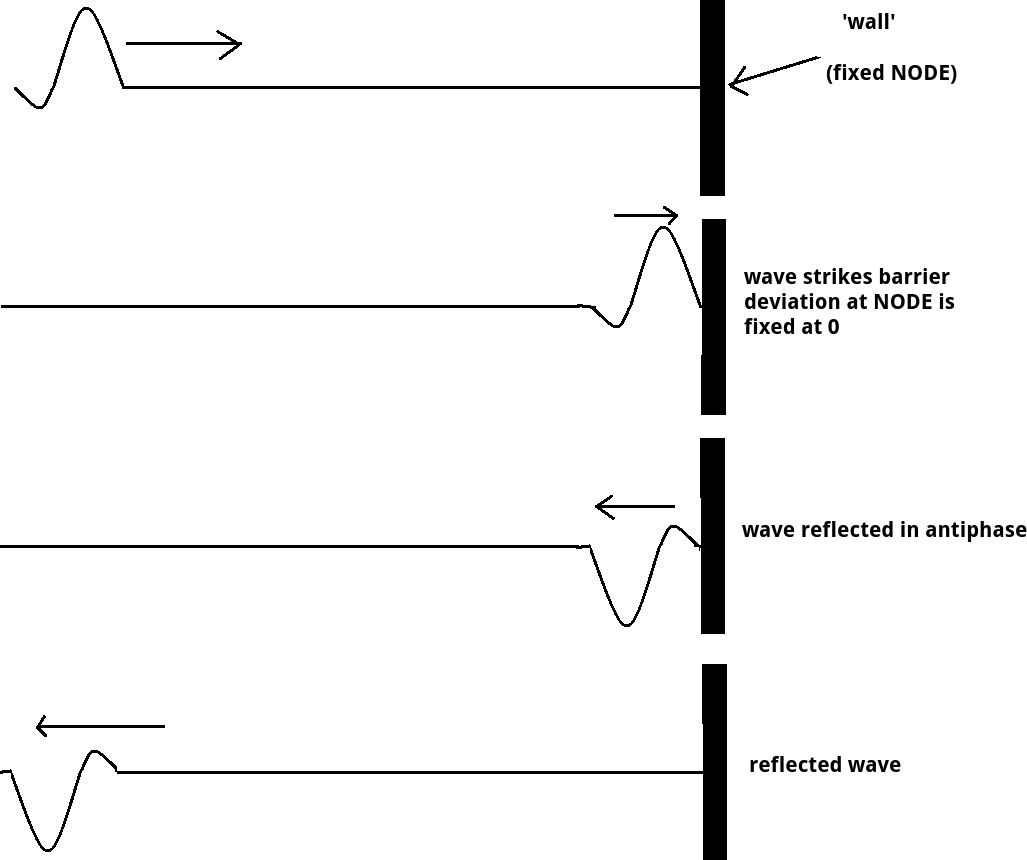
\includegraphics[width=\textwidth]{pictures/closed-circuit-pulse-reflection.png}
            \end{figure}
        \end{column}
    \end{columns}
\end{frame}



\subsection{Donc, pourquoi une impédance?}

\begin{frame}{Pourquoi une impédance}
    \begin{columns}
        \begin{column}{0.5\textwidth}
            \begin{itemize}
                \item Power Factor (efficacité)
                \item Réflections
            \end{itemize}
        \end{column}
        \begin{column}{0.5\textwidth}
            \begin{itemize}
                \item Endommager les composantes
                \item Intégrité du signal
                \item Normes de protocole
            \end{itemize}
        \end{column}
    \end{columns}
    \begin{figure}
        \centering
        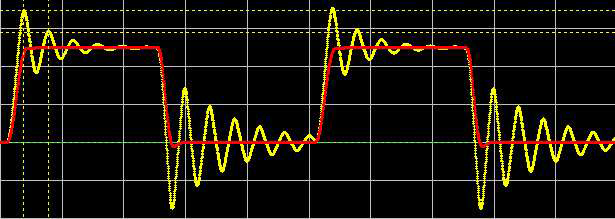
\includegraphics[width=\textwidth]{pictures/impedance-matching-waveform.png}
    \end{figure}
\end{frame}


\subsection{3e impédance cachée!}

\begin{frame}{2 Impédances}
    \resizebox{0.9\textwidth}{!}{
        \begin{circuitikz}[american voltages]
            \draw [thick]
            (0,0) to [short, *-*] (8,0)
            to [open, -*] (8,4)
            (0,0) to [open, v<=$V$] (0,4)
            to [short, *- ,i=$i$] (4,4)
            to [european resistor, l=$Z_0$, a=$50\Omega$] (6, 4)
            to [short, -*] (8,4)
            ;
            \draw[thick, dashed]
            (8, 4) to [short] (8, 3)
            to [short, a=\mbox{$i_L=0A$}] (8, 2)
            to [short, a=\mbox{$Z_L = \infty$}] (8, 1)
            to [short] (8, 0);
        \end{circuitikz}
    }
\end{frame}

\begin{frame}{3 Impédances}
    \resizebox{0.9\textwidth}{!}{
        \begin{circuitikz}[american voltages]
            \draw [thick]
            (0,0) to [short, *-*] (8,0)
            to [open, -*] (8,4)
            (0,0) to [open, v<=$V_S$] (0,4)
            to [short, *-] (0.5, 4)
            to [R, l=$Z_S$, a=$50\Omega$, color=red] (2.5, 4)
            to [short] (4, 4)
            to [european resistor, l=$Z_0$, a=$50\Omega$] (6, 4)
            to [short, -*] (8,4)
            ;
            \draw[thick, dashed]
            (8, 4) to [short] (8, 3)
            to [short, a=\mbox{$i_L=0A$}] (8, 2)
            to [short, a=\mbox{$Z_L = \infty$}] (8, 1)
            to [short] (8, 0);
            \draw[thick, dashed]
            (3, 0.5)
              .. controls (3.5, 1) and (3.5, 3)
              ..node[currarrow, sloped,  allow upside down, pos=1] {}
            (3, 3.5) 
            ;
            \draw
            (4, 0) to [open, l=$V$] (4.25, 4);

        \end{circuitikz}
    }
\end{frame}

\begin{frame}{Matching à la source}
    \begin{columns}
        \begin{column}{0.4\textwidth}
            \begin{itemize}
                \item L'impédance $Z_0$ est en tout point du conducteur
                \item Les points aux bouts doivent êtres matchés
                \item $Z_0 = Z_S = Z_L$
                \bigskip
                \item Réflection à la source possible!
            \end{itemize}
        \end{column}
        \begin{column}{0.6\textwidth}
            \begin{center}
            \resizebox{\textwidth}{!}{
            \begin{circuitikz}[american voltages]
                \draw [thick]
                (0,0) to [short, *-] (8,0)
                to [resistor, l=$Z_L$] (8, 4)
                (0,0) to [open, v<=$V_S$] (0,4)
                to [short, *-] (0.5, 4)
                to [R, l=$Z_S$] (2.5, 4)
                to [short] (4, 4)
                to [european resistor, l=$Z_0$] (6, 4)
                to [short] (8,4)
                ;
                \draw [thick, dashed]
                (3, 0.5)
                  .. controls (3.5, 1) and (3.5, 3)
                  ..node[currarrow, sloped,  allow upside down, pos=1] {}
                (3, 3.5) 
                ;
                \draw
                (4, 0) to [open, l=$V$] (4.25, 4);
            \end{circuitikz}
            }
            \end{center}
        \end{column}
    \end{columns}
\end{frame}
